
\begin{figure*}[h]
    \centering
    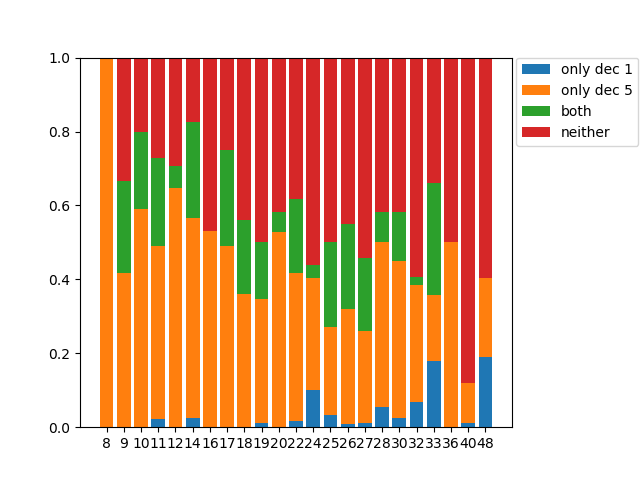
\includegraphics[width=.4\textwidth,keepaspectratio]{figures/jump_subset_out.png}
    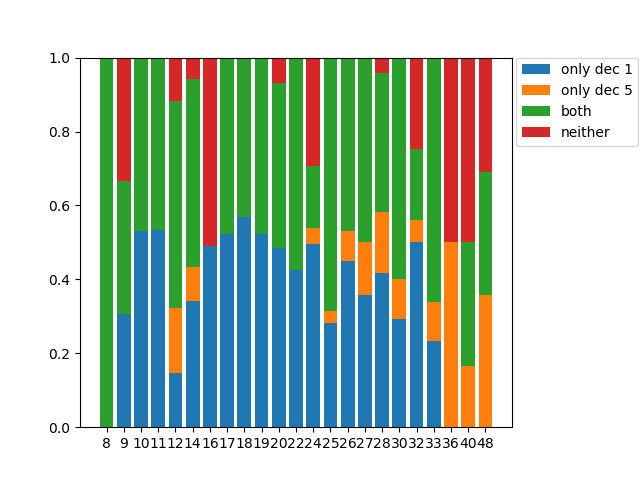
\includegraphics[width=.4\textwidth,keepaspectratio]{figures/template_subset_out.png}
    \caption{Performance distribution for jump and template splits with 5- and 1-decoder widths.}
    \label{fig:kernel_width}
\end{figure*}


\ldots For the random split, we observe the expected pattern in which
both wider encoder and decoder windows lead to perfect
performance. The jump results are less clear-cut, but respect the same
trend: the narrowest encoder-decoder combination achieves the worst
performance, and the widest one the top one. For the around-right
split, it's also better to have the widest encoder, but now we find
that top performance is achieved with the \emph{narrowest} decoder
(width$=$1). Since the novel output sequences in this split are by
construction long, we would have rather expected that models that keep
track of larger window in decoding would have fared better. To gain
some insight on this behaviour, we looked at the performance
distribution across outputs of different (ground-truth) lengths in the
two experiments. Keeping encoder width fixed at 1,
Fig.~\ref{fig:kernel_width} reports the proportions of cases that were
correctly handled only with decoder width 1, 5, with either or
neither. The figure is based on items cases occurring in both data
sets, but the same pattern is confirmed when looking at the whole
generalization sets. We see more cases where both widths worked in
around-right, as expected as we have already established this as an
easier challenge for our CNNs. In general, though, we find that the
wide-decoder jump model behaves quite similarly to the narrow-decoder
around-right model, getting most of its gain from shorter
sequences. One interesting difference is that for around-right we
observe an inversion in performance for the longer sequences, where
actually the wider decoder outperforms the narrower one, in accordance
with our intuition that more context should help longer execution
tasks. Looking qualitatively at the errors, we note that, for both
splits, the narrower decoder needs to skip chunks of commands (e.g.,
executing ``jump around right'' with 3 instead of 4 right turns
followed by jump), whereas the wider kernel seems more likely to
replace commands (e.g., turning left instead of right) than
undershooting the length. Quantitatively, this is supported by the
fact that, for both splits, the narrow kernel errors have considerably
larger variance with respect to ground-truth length. While these
observations confirm the observation that a wider decoder kernel helps
with length management, we still have no insight on why the shorter
kernel should be better on the around-right split. Future work should
pursue a better understanding of how kernel widths affect linguistic
processing in CNNs.

